\documentclass[aspectratio=169]{beamer}

\usepackage{amsmath}
\usepackage{amssymb}
\usepackage{fontspec}
\usepackage{tikz}
\setsansfont{Liberation Sans}
\setmonofont{Liberation Mono}
\usefonttheme{professionalfonts}
\usetheme{Copenhagen}
\setbeamertemplate{navigation symbols}{}
\setbeamertemplate{headline}{}
\setbeamertemplate{footline}[frame number]

\title{Reinforcement Learning}
\subtitle{От своего backpropagation к обучению агентов}
\author{}
\date{}

\begin{document}

\begin{frame}[plain]
  \titlepage
\end{frame}

\begin{frame}{Отправная точка: что уже умеет nn\_lib}
  \begin{itemize}
    \item MLP: линейные слои, ReLU, softmax.
    \item Backpropagation: производная loss проходит через сеть.
    \item Классификация: метка $y$ задаёт направление $p-y$.
  \end{itemize}
  \begin{block}{Новый вопрос}
    В игре никто не сообщает правильное действие.
    Есть только последствия и награды. Откуда взять loss?
  \end{block}
  Цель: вывести первый алгоритм, связать его с библиотекой
  и спроектировать эксперимент на PyTorch с поддержкой GPU.
  Расширять учебную nn\_lib не обязательно.
\end{frame}

\begin{frame}{Твоя идея почти совпадает с REINFORCE}
  \begin{enumerate}
    \item Общая сеть: да, одна policy для многих копий среды.
    \item Вероятности действий: да, softmax и случайная выборка.
    \item Градиент действия: точнее, $\nabla_\theta\log\pi_\theta(a\mid s)$.
    \item Обратная связь: весом служит будущий return,
      позднее --- advantage, а не только знак награды.
  \end{enumerate}
  \begin{block}{Что хранить}
    Проще накапливать наблюдения, действия и награды.
    Градиенты пересчитать после сбора, сохранив те же параметры policy.
  \end{block}
\end{frame}

\begin{frame}{Цикл взаимодействия}
  \centering
  \begin{tikzpicture}[>=stealth, thick]
    \node[draw, rounded corners, minimum width=3cm, minimum height=1cm]
    (agent) at (0,0) {Policy $\pi_\theta$};
    \node[draw, rounded corners, minimum width=3cm, minimum height=1cm]
    (env) at (7,0) {Среда};
    \draw[->] (agent.north) -- ++(0,0.9) -| node[pos=0.25,above]
    {$a_t\sim\pi_\theta(\cdot\mid o_t)$} (env.north);
    \draw[->] (env.south) -- ++(0,-0.9) -| node[pos=0.25,below]
    {$o_{t+1},\ r_t,\ \text{конец эпизода}$} (agent.south);
  \end{tikzpicture}
  \vspace{0.6cm}

  Здесь $r_t$ получена \textbf{после} действия $a_t$.
  Один эпизод: $T$ действий, индексы от $0$ до $T-1$.
\end{frame}

\begin{frame}{State, observation и память}
  \begin{description}
    \item[State $s_t$] Полное состояние мира.
    \item[Observation $o_t$] То, что доступно агенту.
    \item[Markov property] Текущее состояние и действие определяют
      распределение следующего состояния и награды.
  \end{description}
  Позиции недостаточно, если есть инерция: нужна скорость.
  При ограниченном обзоре могут понадобиться история или recurrent policy.
  \begin{block}{Упрощение первого проекта}
    Наблюдение содержит всё необходимое. Ниже пишем $s_t$.
    При конечном лимите ходов включаем оставшееся время.
  \end{block}
\end{frame}

\begin{frame}{Reward --- сейчас; return --- последствия}
  \[
    G_t=\sum_{k=t}^{T-1}\gamma^{k-t}r_k,
    \qquad J(\theta)=\mathbb E_{\tau\sim\pi_\theta}
    \left[\sum_{t=0}^{T-1}\gamma^t r_t\right].
  \]
  $\gamma$ --- discount factor, не learning rate.
  \begin{exampleblock}{Отложенная награда}
    Награды $(0,0,1)$, $\gamma=0.9$:
    returns $(0.81,0.9,1)$.
    Последнее действие не получает всю заслугу.
  \end{exampleblock}
  В первом конечном эксперименте берём $\gamma=1$:
  максимизируем ожидаемую сумму наград эпизода.
\end{frame}

\begin{frame}{Почему обычной классификации недостаточно}
  Выбранное действие не становится правильным только потому,
  что агент его выбрал.
  \[
    L_{\mathrm{CE}}=-\log p_a
    \quad\Longrightarrow\quad
    \frac{\partial L_{\mathrm{CE}}}{\partial z_j}
    =p_j-\mathbf 1[j=a].
  \]
  Без оценки результата такой update подкрепляет любые собственные действия.
  \begin{block}{Идея}
    Увеличивать вероятность действий с хорошими последствиями;
    уменьшать её для действий с результатом хуже ожидаемого.
  \end{block}
\end{frame}

\begin{frame}{Дифференцируем вероятность траектории}
  \small
  Если динамика среды не зависит от параметров $\theta$:
  \[
    p_\theta(\tau)=p(s_0)\prod_t
    \pi_\theta(a_t\mid s_t)P(s_{t+1}\mid s_t,a_t).
  \]
  Используем $\nabla p=p\nabla\log p$:
  \[
    \nabla J=\mathbb E\left[R(\tau)\nabla\log p_\theta(\tau)\right],
    \qquad
    \nabla\log p_\theta(\tau)=\sum_t\nabla\log\pi_\theta(a_t\mid s_t).
  \]
  $R(\tau)=\sum_t\gamma^t r_t$.
  Производные динамики не нужны: игровой движок может быть чёрным ящиком.
  Дискретную выборку действия также не дифференцируем.
\end{frame}

\begin{frame}{От всей траектории к reward-to-go}
  Награды до действия не зависят от него причинно;
  их вклад в ожидаемый градиент равен нулю.
  \[
    \nabla J=\mathbb E\left[\sum_t
    \gamma^t G_t\nabla\log\pi_\theta(a_t\mid s_t)\right].
  \]
  \begin{alertblock}{Следим за соглашениями}
    Для выбранного discounted objective есть внешний $\gamma^t$.
    При $\gamma=1$ он исчезает. В практических алгоритмах встречаются
    другие схемы усреднения; не смешиваем их с этим выводом.
  \end{alertblock}
  Одна траектория даёт шумную оценку. Собираем batch эпизодов.
\end{frame}

\begin{frame}{REINFORCE: loss для знакомого gradient descent}
  Для $B$ полных эпизодов при $\gamma=1$:
  \[
    L_{\mathrm{actor}}=-\frac1B\sum_{i=1}^{B}\sum_t
    \operatorname{stopgrad}(G_{i,t})
    \log\pi_\theta(a_{i,t}\mid s_{i,t}).
  \]
  \begin{itemize}
    \item Награды и returns --- фиксированные численные веса.
    \item Минимизируем loss, значит максимизируем ожидаемый reward.
    \item Делим на число эпизодов: сохраняем сумму вкладов внутри эпизода.
    \item Это surrogate loss; качество измеряем в новых эпизодах.
  \end{itemize}
\end{frame}

\begin{frame}{Мост к backpropagation: всего один множитель}
  Для одного действия с весом $w$:
  \[
    L=-w\log p_a,\qquad
    \boxed{\frac{\partial L}{\partial z_j}
    =w\bigl(p_j-\mathbf1[j=a]\bigr).}
  \]
  Остальная цепочка backpropagation не меняется.
  \begin{exampleblock}{Проверка знака, без batch-нормировки}
    $p=(0.2,0.5,0.3)$, выбрано второе действие, $w=2$.
    Производная $(0.4,-1,0.6)$.
    Gradient descent увеличивает выбранный logit.
    При $w=-2$ направление противоположно.
  \end{exampleblock}
\end{frame}

\begin{frame}{Необязательно: как выглядел бы update в nn\_lib}
  \small
  \begin{itemize}
    \item \texttt{back\_propagation}: вместо $p-y$ нужно $w(p-y)$.
    \item Не передавать $wy$ как метку: $p-wy\ne w(p-y)$.
    \item Накопить batch и вызвать \texttt{apply\_grads} один раз.
      Текущий \texttt{train} обновляет веса при каждом вызове.
    \item Отключить dropout: \texttt{predict} и обучение должны
      пересчитывать одну и ту же policy. Для отладки также отключить L2.
    \item Считать log probability через стабильный log-softmax.
    \item Для critic понадобится линейный выход: softmax одного числа
      всегда равен 1.
  \end{itemize}
  Это мост к знакомому коду. Основной проект использует PyTorch autograd.
\end{frame}

\begin{frame}[fragile]{PyTorch: backprop уже реализован}
  \small
\begin{verbatim}
# policy outputs logits; tensors are on the same device
# batch contains B complete episodes, gamma = 1
probs = torch.distributions.Categorical(logits=policy(obs))
loss = -(probs.log_prob(actions) * returns.detach()).sum() / B
optimizer.zero_grad()
loss.backward()
optimizer.step()
\end{verbatim}
  При сборе: \texttt{no\_grad()} и \texttt{Categorical.sample()}.
  До обработки batch параметры заморожены.
  \begin{block}{CPU / GPU}
    Сеть и batch размещаем на одном device.
    Конкретный пример и настройка устройства есть в конспекте.
  \end{block}
\end{frame}

\begin{frame}[fragile]{Полный первый training loop}
  \small
\begin{verbatim}
repeat:
    freeze policy parameters
    episodes = collect_complete_episodes(B)  # sample actions
    zero_grad()
    for episode in episodes:
        G = 0
        for (obs, action, reward) in reverse(episode):
            G = reward + G                  # gamma = 1
            p = forward(obs)                # same policy
            backward_logits(G * (p - one_hot(action)) / B)
    apply_gradients_once()
    discard episodes
\end{verbatim}
  У среды настоящий конечный горизонт. Returns не пересекают reset.
  Равномерно выбираем reset seeds, не отбрасываем долгие эпизоды.
\end{frame}

\begin{frame}{Почему сначала храним опыт, а не градиенты}
  \begin{itemize}
    \item У каждого действия свой $G_t$.
    \item После суммирования градиентов разные веса уже не восстановить.
    \item Хранить градиент по всем параметрам на каждом шаге дорого.
    \item Наблюдение, действие и награда позволяют повторить forward/backward.
  \end{itemize}
  \begin{block}{Условие корректности простого алгоритма}
    До конца обработки batch веса policy не меняются.
    После update собираем новые данные.
  \end{block}
\end{frame}

\begin{frame}{Baseline: хорошо относительно чего?}
  \[
    V^\pi(s)=\mathbb E[G_t\mid s_t=s],\qquad
    \widehat A_t=G_t-V_\phi(s_t).
  \]
  Ожидали 5, получили 2: advantage $=-3$, даже при положительном return.
  \[
    \mathbb E_{a\sim\pi}[b(s)\nabla\log\pi(a\mid s)]
    =b(s)\nabla\sum_a\pi(a\mid s)=0.
  \]
  Фиксированный baseline, не зависящий от выбранного действия,
  не меняет ожидаемый градиент и может уменьшить дисперсию.
  Начни со среднего return предыдущих batches.
\end{frame}

\begin{frame}{Actor и critic: две задачи обучения}
  \begin{description}
    \item[Actor $\pi_\theta$] Выбирает действие.
    \item[Critic $V_\phi$] Предсказывает будущий return текущей policy.
  \end{description}
  \[
    L_{\mathrm{actor}}=-\frac1B\sum_{i,t}
    \operatorname{stopgrad}(\widehat A_{i,t})\log\pi_\theta(a_{i,t}\mid s_{i,t}),
  \]
  \[
    L_{\mathrm{value}}=\frac{1}{2N}\sum_{i,t}
    \bigl(V_\phi(s_{i,t})-\operatorname{stopgrad}(G_{i,t})\bigr)^2.
  \]
  $N$ --- число переходов. Сначала две отдельные сети.
  Веса actor вычислить старым critic до обучения на текущем batch.
\end{frame}

\begin{frame}{TD: не обязательно ждать конца эпизода}
  \[
    y_t=r_t+\gamma(1-\mathrm{terminated}_t)V_{\mathrm{old}}(s_{t+1}),
    \qquad\delta_t=y_t-V_{\mathrm{old}}(s_t).
  \]
  \begin{itemize}
    \item Monte Carlo: фактический полный return; высокая дисперсия.
    \item Temporal difference: reward плюс оценка продолжения.
    \item Bootstrapping снижает зависимость от полного исхода,
      но неточный critic вносит смещение.
    \item Targets фиксированы при обновлении; $\delta_t$ можно
      использовать как оценку advantage.
  \end{itemize}
\end{frame}

\begin{frame}{Окончание задачи и остановка сбора --- разные события}
  \begin{description}
    \item[Terminated] Задача закончилась: bootstrap равен нулю.
    \item[Truncated] Внешний обрыв: используем value последнего
      наблюдения до reset.
  \end{description}
  \begin{block}{Лимит времени}
    Если 40 ходов --- правило игры, это termination;
    оставшееся время входит в observation.
    Если остановился только сбор данных, это truncation.
  \end{block}
  При обоих флагах termination имеет приоритет.
  REINFORCE без critic сначала использует только полные эпизоды.
\end{frame}

\begin{frame}{GAE: соединить несколько TD-оценок}
  \[
    \widehat A_t=\delta_t+\gamma\lambda c_t\widehat A_{t+1}.
  \]
  \begin{itemize}
    \item $\lambda$ регулирует компромисс смещения и дисперсии.
    \item $c_t=0$ на границе эпизода или rollout batch.
    \item На внешнем обрыве TD сохраняет bootstrap, но рекурсия
      advantage не пересекает reset.
    \item При $\lambda=0$ остаётся одношаговый TD residual.
    \item При $\lambda=1$ и полном эпизоде сумма даёт $G_t-V(s_t)$.
  \end{itemize}
  Реализовать после рабочей Monte Carlo версии с baseline.
\end{frame}

\begin{frame}{Почему нельзя бесконечно учиться на старом batch}
  \textbf{On-policy}: данные собраны policy, градиент которой оцениваем.
  После update вероятности действий и распределение посещаемых состояний
  меняются.
  \begin{itemize}
    \item REINFORCE: один batch, один update, новый опыт.
    \item PPO: несколько epochs на свежем batch с поправкой objective.
    \item Off-policy методы специально устроены для использования
      опыта другой policy; пример --- DQN с replay buffer.
  \end{itemize}
  Обычный многократный \texttt{train} на прежних эпизодах не превращает
  REINFORCE в PPO.
\end{frame}

\begin{frame}{PPO: следующий этап, а не первый}
  \small
  Сохраняем старые log probabilities и advantages:
  \[
    \rho_t(\theta)=\exp\bigl(\log\pi_\theta(a_t\mid s_t)
    -\log\pi_{\mathrm{old}}(a_t\mid s_t)\bigr),
  \]
  \[
    L_{\mathrm{clip}}=-\mathbb E_t\left[
      \min\left(\rho_t\widehat A_t,
      \operatorname{clip}(\rho_t,1-\epsilon,1+\epsilon)\widehat A_t\right)
    \right].
  \]
  Ограничиваем стимул слишком сильно менять вероятности на старом batch.
  Clipping не гарантирует жёсткую границу изменения policy.
  Контролируем KL divergence, entropy и clip fraction.
  \begin{block}{Практический порядок}
    REINFORCE $\rightarrow$ baseline $\rightarrow$ actor--critic
    $\rightarrow$ GAE $\rightarrow$ PPO.
  \end{block}
\end{frame}

\begin{frame}{Где другие направления RL}
  \small
  \begin{description}
    \item[Policy gradient] Непосредственно учим вероятности действий.
    \item[Q-learning / DQN] Учим $Q(s,a)$ --- ожидаемый return
      после действия; нужны exploration и Bellman targets.
    \item[Actor--critic] Совмещаем policy и оценку ценности.
      PPO и SAC относятся к этому широкому направлению.
    \item[Model-based] Учим или используем модель динамики и планируем.
  \end{description}
  Для непрерывного управления возможна Gaussian policy вместо softmax.
  Это потребует другого log probability и обработки границ действий.
  Первый проект оставляем дискретным.
\end{frame}

\begin{frame}{Первый проект: сетка 7\,$\times$\,7}
  \small
  \begin{columns}
    \begin{column}{0.34\textwidth}
      \centering
      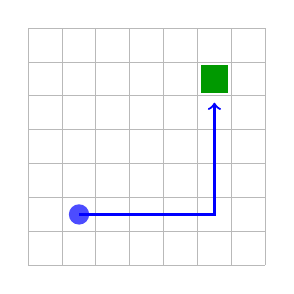
\begin{tikzpicture}[scale=0.43]
        \draw[step=1,gray!55] (0,0) grid (7,7);
        \fill[blue!70] (1.5,1.5) circle (0.3);
        \fill[green!60!black] (5.1,5.1) rectangle (5.9,5.9);
        \draw[->,thick,blue] (1.5,1.5) -- (5.5,1.5) -- (5.5,4.8);
      \end{tikzpicture}
    \end{column}
    \begin{column}{0.64\textwidth}
      Разные старт и цель, без препятствий и инерции.
      \begin{itemize}
        \item 4 действия; выход за стену тратит ход.
        \item Не больше 40 ходов --- правило задачи.
        \item $+1$ за цель, $-0.01$ за любой другой ход.
        \item Observation: координаты агента, цели и время.
        \item MLP $5\to32\to32\to4$, $\gamma=1$.
      \end{itemize}
    \end{column}
  \end{columns}
  \vspace{0.2cm}
  Ручная policy достигает цели максимум за 12 ходов:
  используем её для проверки среды.
\end{frame}

\begin{frame}[fragile]{Контракт с игровым движком}
\begin{verbatim}
reset(seed) -> observation, info
step(action) -> observation, reward,
                terminated, truncated, info
\end{verbatim}
  \begin{itemize}
    \item Среда владеет физикой, состоянием, reward и reset.
    \item Тренер владеет сетью, optimizer и batch.
    \item Action соответствует фиксированному числу physics ticks.
    \item Рендеринг не влияет на simulation timestep.
    \item В headless режиме те же правила, больше шагов в секунду.
  \end{itemize}
  Сначала один процесс; IPC и batch-команды добавлять по необходимости.
\end{frame}

\begin{frame}{Общая сеть: две разные постановки}
  \begin{block}{Независимые среды}
    Много копий одной задачи собирают траектории общей policy.
    Это первый вариант: свои reset, rewards и returns у каждой копии.
  \end{block}
  \begin{block}{Общая арена}
    Агенты влияют друг на друга. Нужны правила общей/личной награды,
    наблюдений и распределения заслуги. Возникает multi-agent RL.
  \end{block}
  В \texttt{NN} есть изменяемые forward-буферы: один объект нельзя
  одновременно вызывать из разных потоков без изменения архитектуры.
\end{frame}

\begin{frame}{Маршрут реализации с проверками}
  \small
  \begin{enumerate}
    \item Bandit: один шаг, три действия, проверить знак и gradient check.
    \item Сетка: REINFORCE на полных эпизодах, random baseline.
    \item Baseline и critic: сравнить при одинаковом бюджете шагов.
    \item TD и GAE: вручную проверить targets и границы эпизодов.
    \item Движок: сначала ручной агент, затем обучение без рендера.
    \item Готовый PPO из Stable-Baselines3; при разборе проверить $\rho=1$ до update и оба знака advantage.
    \item Независимые арены; затем взаимодействующие агенты.
  \end{enumerate}
  Каждый этап должен работать отдельно до добавления следующего.
\end{frame}

\begin{frame}{Готовый стек для проекта}
  \begin{enumerate}
    \item PyTorch: короткий учебный REINFORCE, готовые autograd и Adam.
    \item Gymnasium: первая среда и стандартный контракт.
    \item Stable-Baselines3: готовый PPO для более сложной задачи.
    \item Godot RL Agents: готовый мост между движком и Python.
  \end{enumerate}
  TorchRL --- альтернатива для более детального управления компонентами.
  Свой PPO, IPC и GPU kernels не обязательны для первого проекта.
  \begin{block}{Разделение ответственности}
    Python обучает сеть; движок симулирует мир и показывает поведение.
  \end{block}
\end{frame}

\begin{frame}{GPU ускоряет сеть, но не весь эксперимент}
  \begin{itemize}
    \item На GPU: батчевый forward, backward, optimizer.
    \item Физика обычной Godot-среды автоматически туда не переносится.
    \item Маленькая MLP может работать быстрее на CPU из-за накладных затрат.
    \item Больше независимых сред помогает собирать batch;
      скорость ограничивается также физикой и обменом данными.
  \end{itemize}
  Измеряем steps/s, время сбора и время update на CPU и GPU.
  Для PPO с MLP документация SB3 рекомендует рассмотреть CPU.
  \begin{block}{Выбор оборудования следует из измерений}
    Поддержка GPU в стеке есть; обещать ускорение для любой среды нельзя.
  \end{block}
\end{frame}

\begin{frame}{Что считать успехом эксперимента}
  Предлагаемый критерий для сетки:
  \begin{itemize}
    \item 90\% успехов на 500 evaluation seeds.
    \item Критерий выполнен у 4 из 5 независимо обученных моделей.
    \item Первый бюджет --- миллион взаимодействий, затем анализ.
    \item Отдельно измерять stochastic и greedy policy.
  \end{itemize}
  Логировать success rate, return, длину эпизода, entropy,
  gradient norm и число шагов среды.
  Сохранять seed, конфигурацию, checkpoint и replay.
  \begin{block}{Не путать метрики}
    Падение actor loss не доказывает улучшение поведения.
  \end{block}
\end{frame}

\begin{frame}{Типичные поломки и что проверять}
  \small
  \begin{description}
    \item[Не учится даже bandit] Знак update, вес всего $p-y$, sampling.
    \item[Учится только одному действию] Entropy, размер шага,
      распределение наград, exploration.
    \item[Награда растёт, цель не достигается] Агент оптимизирует
      reward, а не наше намерение: проверить обходные стратегии.
    \item[Ломается после reset] Returns/GAE пересекли эпизоды
      или bootstrap взят от нового стартового состояния.
    \item[Работает только один seed] Оценить разброс, бюджет и настройки.
    \item[Не сходится в движке] Сначала проверить observation,
      физические шаги и ручную policy.
  \end{description}
\end{frame}

\begin{frame}{Вопросы для самопроверки}
  \begin{enumerate}
    \item Почему нужен $\log\pi(a\mid s)$, а не градиент действия?
    \item Почему награда $+2$ может уменьшить вероятность действия?
    \item Почему нельзя передать $w\cdot\mathrm{one\_hot}(a)$ в старый train?
    \item Почему softmax с одним выходом не годится для critic?
    \item Когда timeout требует bootstrap?
    \item Почему общий replay buffer не делает REINFORCE off-policy?
  \end{enumerate}
  Выводы, ответы и подробная спецификация проекта:
  \texttt{presentations/rl/README.md}.
\end{frame}

\begin{frame}{Источники и дальнейшее чтение}
  \small
  \begin{enumerate}
    \item Sutton \& Barto,
      \href{http://incompleteideas.net/book/the-book-2nd.html}
      {Reinforcement Learning: An Introduction}.
      Главы 2--3, 6, 13.
    \item \href{https://spinningup.openai.com/en/latest/spinningup/rl_intro3.html}
      {Spinning Up: Intro to Policy Optimization}.
      Вывод policy gradient и reward-to-go.
    \item \href{https://gymnasium.farama.org/main/tutorials/handling_time_limits/}
      {Gymnasium: Handling Time Limits}.
      Termination, truncation и bootstrap.
    \item Schulman et al.,
      \href{https://arxiv.org/abs/1506.02438}{Generalized Advantage Estimation}.
    \item Schulman et al.,
      \href{https://arxiv.org/abs/1707.06347}{Proximal Policy Optimization Algorithms}.
  \end{enumerate}
  Сначала вывести и реализовать REINFORCE; статьи про GAE и PPO
  читать после первого работающего агента.
\end{frame}

\begin{frame}{Документация готовых инструментов}
  \begin{itemize}
    \item \href{https://docs.pytorch.org/docs/stable/distributions.html\#categorical}
      {PyTorch: Categorical} --- sampling и log probability.
    \item \href{https://stable-baselines3.readthedocs.io/en/stable/modules/ppo.html}
      {Stable-Baselines3: PPO} --- API, параметры, CPU/GPU.
    \item \href{https://github.com/edbeeching/godot_rl_agents}
      {Godot RL Agents} --- интеграция среды с Python.
    \item \href{https://docs.pytorch.org/tutorials/intermediate/reinforcement_ppo.html}
      {TorchRL: PPO tutorial} --- альтернативный путь к компонентам алгоритма.
  \end{itemize}
  Версии зависимостей фиксировать при создании проекта.
  Конспект содержит примеры PyTorch update и подключения готового PPO.
\end{frame}

\end{document}
